

\documentclass[polish]{beamer}
\usepackage{babel}
 
\usepackage[utf8]{inputenc}
\usepackage[T1]{fontenc}
 
 
%Information to be included in the title page:
\title{Weryfikacja możliwości sterowania łazikiem za pomocą sieci neuronowych}
\author{Paweł Dybiec}
%\institute{II UWr}
\date{2018}
 
 
\usetheme{Warsaw} 

\begin{document}
 
\frame{\titlepage}
 
\begin{frame}
\frametitle{Problem}
\begin{figure}
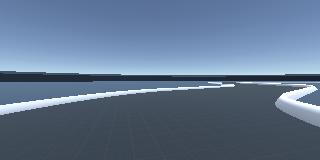
\includegraphics[width=0.475\textwidth]{sim.jpg}%
\hfill   

\includegraphics[width=0.475\textwidth]{nakaz_skretu.png}
\end{figure}
\end{frame}

\begin{frame}
\frametitle{Rozwiązanie}
Konwolucyjna sieć neuronowa 
\begin{figure}
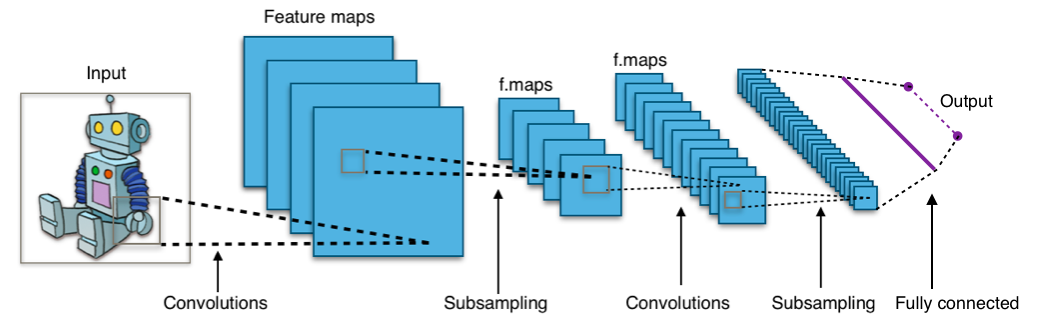
\includegraphics[width=\textwidth]{Typical_cnn.png}
\caption{Źródło: \href{https://commons.wikimedia.org/wiki/File:Typical\_cnn.png}{https://commons.wikimedia.org/wiki/File:Typical\_cnn.png}}
\end{figure}
\end{frame}

\begin{frame}
\frametitle{Trening i dane}
\framesubtitle{Symulator}
Dlaczego symulator?
\pause
\begin{itemize}
\item Szybkość zbierania danych
\item Bezpieczeństwo
\item Prostota
\end{itemize}
\pause
Dane:
\begin{itemize}
\item 3 kamery
\item 50 minut nagrań
\item lustrzane odbicie
\end{itemize}
\end{frame}

\begin{frame}
\frametitle{Trening i dane}
\framesubtitle{Łazik}
Dane:
\begin{itemize}
\item Kierunek jazdy nadal jednoznaczny
\item 150GB
\item 1 kamera + lustrzane odbicie
\end{itemize}
\end{frame}

\begin{frame}
\frametitle{Przejazdy}
Symulator, uczony na przejazdach tylko w jedną stronę $\rightarrow$ potrafi też w drugą

Łazik $\rightarrow$ potrafi objechać garaż instytutu
\pause

Demo na symulatorze

\end{frame}

\begin{frame}
\frametitle{Reakcje na obraz}
\framesubtitle{Symulator}
\begin{center}
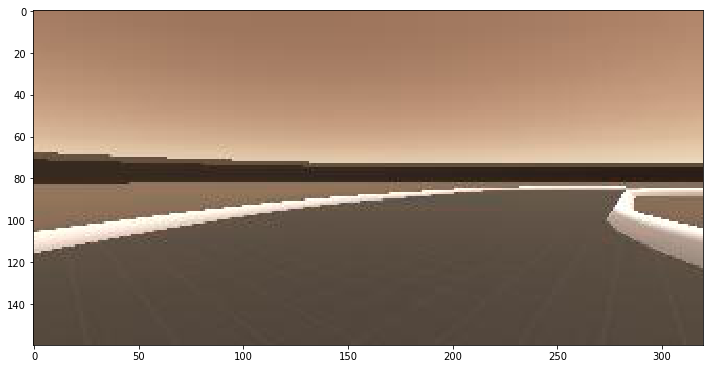
\includegraphics[height=0.42\textheight]{sim_img.png}
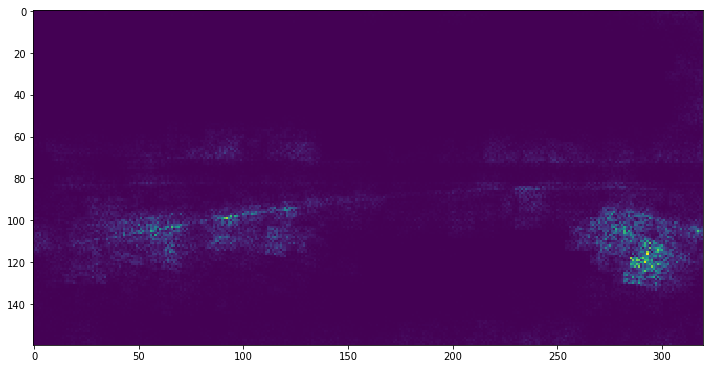
\includegraphics[height=0.42\textheight]{sim_img_act.png}
\end{center}
\end{frame}

\begin{frame}
\frametitle{Reakcje na obraz}
\framesubtitle{Łazik}
\begin{center}
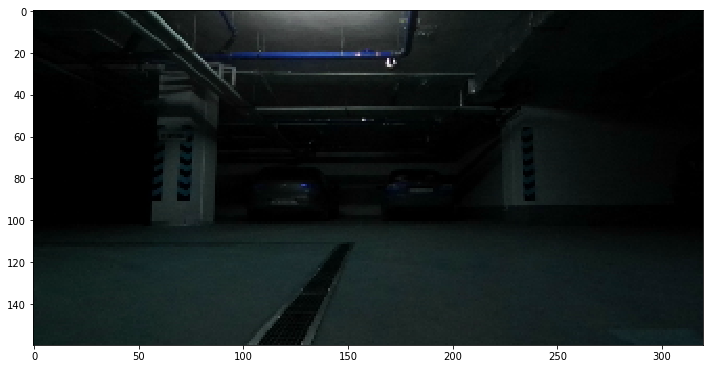
\includegraphics[height=0.42\textheight]{real_img.png}
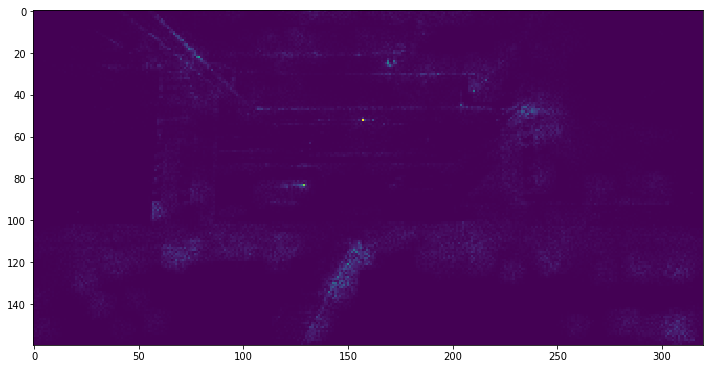
\includegraphics[height=0.42\textheight]{real_img_act.png}
\end{center}
\end{frame}

\begin{frame}
\frametitle{Porównanie do kierowcy}
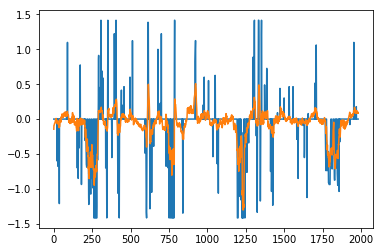
\includegraphics[width=0.9\textwidth]{real_data_ang.png}
\begin{itemize}
\item Mniej gwałtowne
\item Podobne reakcje
\end{itemize}
\end{frame}

\begin{frame}
\frametitle{Co dalej}
\begin{itemize}
\item Przetwarzanie kilku ostatnich obrazków
\item Rekurencyjna sieć neuronowa
\item Reinforcement learning
\end{itemize}
\end{frame}
\end{document}

